\documentclass[10pt]{article}
\usepackage{icmlko}

\icmlmeta{IP 파운데이션 월드모델}{202}{재는 것을 먼저, 바꾸는 것을 나중에}{노트 201이 ``도메인 선택은 최근 가중 위에서 잉여''로 닫으며 순서를 뒤집어 보라고 적었다. 뒤집었더니 잉여가 아니었다 --- 가중이 재는 눈을 가리고 있었다}

\begin{document}

\twocolumn[
\icmlheader

\begin{abstract}
노트 201이 최근 가중을 먼저 걸고 도메인 선택을 나중에 해서 ``선택은
$+$0.0007($t{=}0.13$)로 잉여''라고 적고, ``순서를 뒤집어 재는 것이 이 노트를
반증하거나 굳힌다''로 닫았다. \textbf{반증됐다.} 선택을 먼저 하고 가중을
나중에 걸면 판이 $+$0.4043 에서 \textbf{$+$0.4094} 가 되고($+$0.0053 ·
$t{=}1.25$), 선택의 한계 기여가 $+$0.0007 에서 \textbf{$+$0.0059}
($t{=}1.81$)로 살아난다. \textbf{까닭은 재는 눈이다.} 도메인 선택은 ``혼자
모형이 풀링보다 나은가''를 안쪽에서 재서 정하는데, \emph{가중한} 자료에서
재면 모바일의 격차가 $+$0.143 에서 \textbf{$+$0.004} 로 지워진다 --- 최근
가중이 이미 그 도메인을 구해 놓아서 더 잴 것이 없어 보이는 것이다. 그런데
\emph{최종} 모형에서는 여전히 혼자 쪽이 낫다. \textbf{가중이 신호를 없앤
것이 아니라 신호를 \emph{보는 눈}을 가린 것이다.} 도메인별로 보면 이
차이가 통째로 \textbf{모바일 하나}에 있다($+$0.0344) --- 나머지 여덟은
소수 넷째 자리까지 정확히 0 이다. \textbf{규약으로 적는다: 손잡이를 순차로
고를 때 \emph{재는} 손잡이를 먼저, \emph{바꾸는} 손잡이를 나중에.} 노트 195가
``같이 고르지 말고 순차로''를 세웠는데 순서까지는 안 정했고, 이 노트가
그것을 채운다. 등록 형태의 순서 기본값을 ``선택 먼저''로 바꿨다. 지금
포트폴리오는 챔피언 \texttt{F18\_bagboost} $+$0.4490, \texttt{F8\_boost}
$+$0.4404, \textbf{\texttt{F21\_recentpick} $+$0.4094}(선형 최고),
\texttt{F6\_directpool\_recent} $+$0.4004 이고, \textbf{챔피언과 선형의
격차가 0.078 에서 0.040 으로 줄었다.}
\end{abstract}
]

\begin{figure*}[t]
\centering
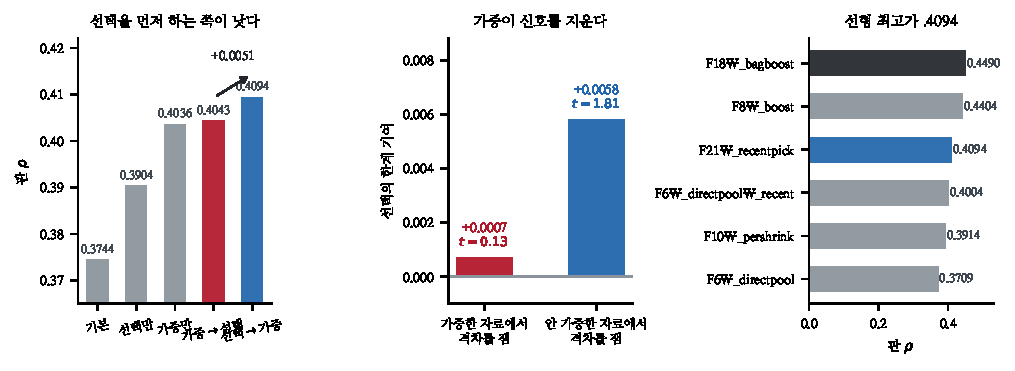
\includegraphics[width=\textwidth]{figs/order2.pdf}
\caption{왼쪽 --- 선택을 먼저 하는 쪽이 낫다. 가운데 --- 가중이 신호를
지운다. 오른쪽 --- 선형 최고가 .4094.}
\end{figure*}

\section{순서가 답을 바꾼다}

\begin{table}[t]
\centering\tsize
\caption{두 손잡이, 두 순서. $\alpha{=}20$ 고정.}
\begin{tabular}{lrl}
\toprule
& 판 $\rho$ & \\
\midrule
기본 (가중 X · 선택 X) & .3744 & \\
선택만 & .3904 & $+$.0160 \\
가중만 & .4036 & $+$.0292 \\
\midrule
가중 $\to$ 선택 & .4043 & 선택 $+$.0007 \\
\textbf{선택 $\to$ 가중} & \textbf{.4094} & \textbf{선택 $+$.0059} \\
\bottomrule
\end{tabular}
\end{table}

\claimx{\textbf{선택을 먼저 하면 $+$0.0053 더 좋다}($t{=}1.25$). 그리고
선택의 한계 기여가 $+$0.0007($t{=}0.13$)에서 $+$0.0059($t{=}1.81$)로
살아난다.}{\textbf{노트 201의 ``잉여''는 순서 탓이었다} --- 그 노트가 걸어
둔 대로 순서를 뒤집으니 결론이 뒤집혔다.}

\section{가중이 재는 눈을 가린다}

\begin{table}[t]
\centering\tsize
\caption{안쪽 격차(혼자 $-$ 풀링). 문턱 0.02.}
\begin{tabular}{lrr}
\toprule
& 가중 없이 잼 & $\tau{=}2$ 로 잼 \\
\midrule
\textbf{모바일} & \textbf{$+$.143} & \textbf{$+$.004} \\
만화 & $+$.020 & $-$.012 \\
세계애니 & $+$.004 & $-$.000 \\
웹툰 & $-$.012 & $+$.002 \\
\midrule
혼자로 고르는 것 & 만화·모바일 & 펀딩 \\
\bottomrule
\end{tabular}
\end{table}

\claimx{\textbf{모바일의 격차가 지워진다}($+$0.143 $\to$ $+$0.004). 노트
201은 이것을 ``가중이 이미 그 일을 했다''로 읽었는데, \textbf{최종 모형에서는
여전히 혼자 쪽이 낫다}($+$0.0344).}{그러니 가중이 신호를 \emph{없앤} 것이
아니라 신호를 \emph{보는 눈}을 가린 것이다. 되뽑기가 안쪽 학습의 서로 다른
행을 63\%로 줄이고(노트 196), 그 흐림이 격차 추정을 뭉갠다.}

\claimx{\textbf{차이가 통째로 모바일 하나에 있다.} 도메인 아홉 중 여덟이
소수 넷째 자리까지 정확히 0 이고 모바일만 $+$0.0344 다.}{노트 197에서도
이 이득의 93\%가 모바일이었다 --- \textbf{같은 도메인이 세 노트 연속으로
혼자 일한다.} 모바일은 유보 441건에 혼자 $\rho$ 가 $+$0.514 로 자기 자료로
제일 잘 배우는 도메인이다.}

\section{규약}

\claimx{\textbf{손잡이를 순차로 고를 때 \emph{재는} 손잡이를 먼저,
\emph{바꾸는} 손잡이를 나중에.} 선택은 자료를 재서 정하고 가중은 자료를
바꾼다 --- 바꾸고 나서 재면 못 본다.}{노트 195가 ``같이 고르지 말고
순차로''를 세웠는데 \textbf{순서까지는 안 정했다.} 이 노트가 그것을 채운다
--- 그리고 이 규약은 안쪽만 보고 지킬 수 있다.}

\claimx{일반화가 어디까지인지는 모른다. 여기서 ``재는'' 손잡이는 도메인
선택 하나이고 ``바꾸는'' 손잡이는 최근 가중 하나다. \textbf{둘 다 재는
손잡이거나 둘 다 바꾸는 손잡이면 순서가 어떤지는 안 쟀다.}}{다만 노트
189의 알파는 ``바꾸는'' 쪽이 아니라 모형 손잡이라 이 규약 바깥이다 ---
알파와 가중을 같이 고르는 것은 노트 195에서 이미 나빴다.}

\begin{table}[t]
\centering\tsize
\caption{지금 포트폴리오.}
\begin{tabular}{lrl}
\toprule
& 판 $\rho$ & \\
\midrule
\textbf{F18 배깅} & \textbf{.4490} & 챔피언 \\
F8 부스트 & .4404 & \\
\textbf{F21 최근·선택} & \textbf{.4094} & \textbf{선형 최고} \\
F6 능형 최근 & .4004 & \\
F10 도메인별 & .3914 & \\
F6 능형 & .3709 & \\
\bottomrule
\end{tabular}
\end{table}

\claimx{\textbf{챔피언과 선형의 격차가 0.078 에서 0.040 으로 줄었다.} 노트
185가 ``공유 축에서는 선형이 트리와 대등하다''를 보였고, 전체 축에서도
절반으로 좁혔다.}{남은 0.040 이 노트 186$\sim$188 이 잰 ``트리는 무리 안에서
곱하고 무리를 가로질러 조건한다''일 것이다 --- \textbf{그쪽은 명시로 옮겨
담는 데 아홉 번 실패했다.}}

\begin{table}[t]
\centering\tsize
\caption{남은 것.}
\begin{tabular}{ll}
\toprule
\textbf{트리} & 최근 가중을 F18 에 --- 규약이 막고 있다 \\
모바일 & 세 노트 연속 혼자 일한다 --- 왜 \\
순서 규약 & 재는 손잡이가 둘일 때는 \\
\bottomrule
\end{tabular}
\end{table}

두 번째 줄이 곧바로 잴 수 있고 이 흐름에서 자주 나온 이름이다. 모바일은
노트 197 · 201 · 202 에서 연속으로 ``풀에서 빼야 하는 유일한 도메인''이었고,
혼자 $\rho$ 가 $+$0.514 로 제일 높다. \textbf{왜 그 도메인만 자기 자료로 잘
배우나} --- 유보 441건에 축 열아홉이 다 차 있고(덮음 100\%), 라벨이 앱스토어
순위라 다른 도메인보다 잡음이 적을 수 있다. \textbf{그것이 맞으면 ``자기
자료로 배울 수 있는 조건''을 미리 알 수 있고, 새 도메인을 들일 때 풀에
넣을지 말지를 자료를 보기 전에 정할 수 있다.}

\end{document}
